\documentclass{article}

\usepackage[a4paper, total={6.5in, 10in}]{geometry}
\usepackage{xurl}
\usepackage{listings}
\usepackage{graphicx}
\usepackage{float}

\title{Performance Comparison Between Different Concurrent Lists}
\author{
    Claudio Scheer\\
    claudio.scheer@edu.pucrs.br
}
\date{\today}

\begin{document}

\maketitle

\section{Introduction}

In this report, I will present performance results using different list approaches. Five approaches were tested: coarse list, fine list, lazy list, lock free list and optimistic list. Each of these concurrent lists has methods for adding items, removing items, and testing whether the list contains a specific item.

To assess performance, I used the implementations provided by the authors of the book \cite{DBLP:books/daglib/0020056}. These implementations needed a few changes discussed in Section~\ref{section:list_problems}. As all implementations were in Java, I also executed all tests in Java.

I do not discuss in depth the differences between the lists in this report, as these differences are discussed in detail in Section 9 of the book \cite{DBLP:books/daglib/0020056}. In addition, the differences and how each list is implemented were widely discussed in class.

In doing so, in Section~\ref{section:methodology}, I discussed the methodology used in the tests and, in Section~\ref{section:results}, I present the results of the tests.


\section{Problems with the authors' implementation} \label{section:list_problems}

Two main problems were found: an implementation error in the optimistic list and outdated implementations. All implementations were downloaded from this website: \url{https://booksite.elsevier.com/9780123973375}.

In the provided implementation of the optimistic list (\texttt{OptimisticList.java}), authors use the following method to add an item to the list:

\begin{lstlisting}[language=Java, numbers=left, captionpos=b, basicstyle=\ttfamily\footnotesize, caption=Method add of OptimisticList.java, label=lst:add_optimistic]
public boolean add(T item) {
    int key = item.hashCode();
    while (true) {
        Entry pred = this.head;
        Entry curr = pred.next;
        while (curr.key <= key) {
            pred = curr;
            curr = curr.next;
        }
        pred.lock();
        curr.lock();
        try {
            if (validate(pred, curr)) {
                if (curr.key == key) { // present
                    return false;
                } else { // not present
                    Entry entry = new Entry(item);
                    entry.next = curr;
                    pred.next = entry;
                    return true;
                }
            }
        } finally { // always unlock
            pred.unlock();
            curr.unlock();
        }
    }
}
\end{lstlisting}

On lines 7 and 8, the \texttt{pred} variable assumes the current node and \texttt{curr} assumes the next node. Therefore, if the \texttt{=} sign is used on line 6 of Listing~\ref{lst:add_optimistic}, the test on line 14 will never be satisfied and the item will always be added to the list. Hence, to solve this problem, I simply removed the \texttt{=} sign on line 6.

Another problem I had with the lists was the different implementations between the 2008 and 2012 book edition. In the 2012 edition, some implementations were updated, but the source code provided was not. Therefore, all implementations were updated according to the 2012 book edition.

The next point is not a problem with the list's implementations, but a necessary feature for my tests. The required feature was a method that could return the size of the list. This method was used to test whether the list size was stable during the test period.

Therefore, to avoid adding an overhead to the methods originaly implemented by the authors, I create a method that simply looks for the next item from the head node to the tail node. The nodes are counted and the the count is returned. All lists follow the same logic. This method has no blocking, which can make the return of this method out of date. However, in my tests, this did not appear to be a problem.


\section{Testing methodology} \label{section:methodology}

The experiments were run on a computer with the following configuration:

\begin{itemize}
    \item \textbf{Java version}: openjdk 14.0.1
    \item \textbf{OS}: Ubuntu 20.04
    \item \textbf{Cores per socket}: 6
    \item \textbf{Threads per core}: 2
    \item \textbf{CPUs}: 12
    \item \textbf{RAM}: 32GB
\end{itemize}

Since the computer has 12 CPUs available, I ran the experiments using 2, 4, 6, 8, 10 and 12 threads. For each number of threads, I tested three list sizes: 100 items, 1000 items and 10000 items. These eighteen experiments were executed three time each and the mean and standard deviation were used to analyze the results.

The number of elements in the list must be stable. Therefore, as the number added and removed from the list is random, I generated random numbers using Equation~\ref{eq:random_number}, where $N$ is the size of the list.

\begin{equation} \label{eq:random_number}
    0 \leq x < (N * 2)
\end{equation}

There are four possible operations to be performed on a list: add, remove, contains and list size. The list size operation is used to colect the size of the list at a specific point. The probability of each operation is 40\%, 40\%, 19.9999\% and 0.0001\%, respectively.

In summary, the specific number of threads is started and each thread gets a random operation and performs it. The number of operations performed on each thread is stored and added to other threads at the end of the test.

The warm-up and test time was 15 seconds and 60 seconds, respectively. The operations performed were counted only during the test time. To obtain the throughput of each list, I divided the total number of operations performed on all threads by the test time. In the throughput, the test time also includes the time to interrupt and join the threads.


\section{Results} \label{section:results}

Each section below shows the throughput and the list size for each list tested. The throughput plot shows the average value and the standard deviation, separated by the $-$ (hyphen) character.

In general, the smaller the list size, the higher the throughput. In addition, in all implementations of the lists, the size remained stable. Since the list size is stable, I do not show the number of each operation performed in this report. However, all of this information can be seen in the GitHub repository, presented in Section~\ref{sec:source-code}, in the folder \texttt{test/raw-data}.

\subsection{Coarse list}

Figure~\ref{fig:coarse-size} shows the average size of the coarse list.

\begin{figure}[H]
    \centering
    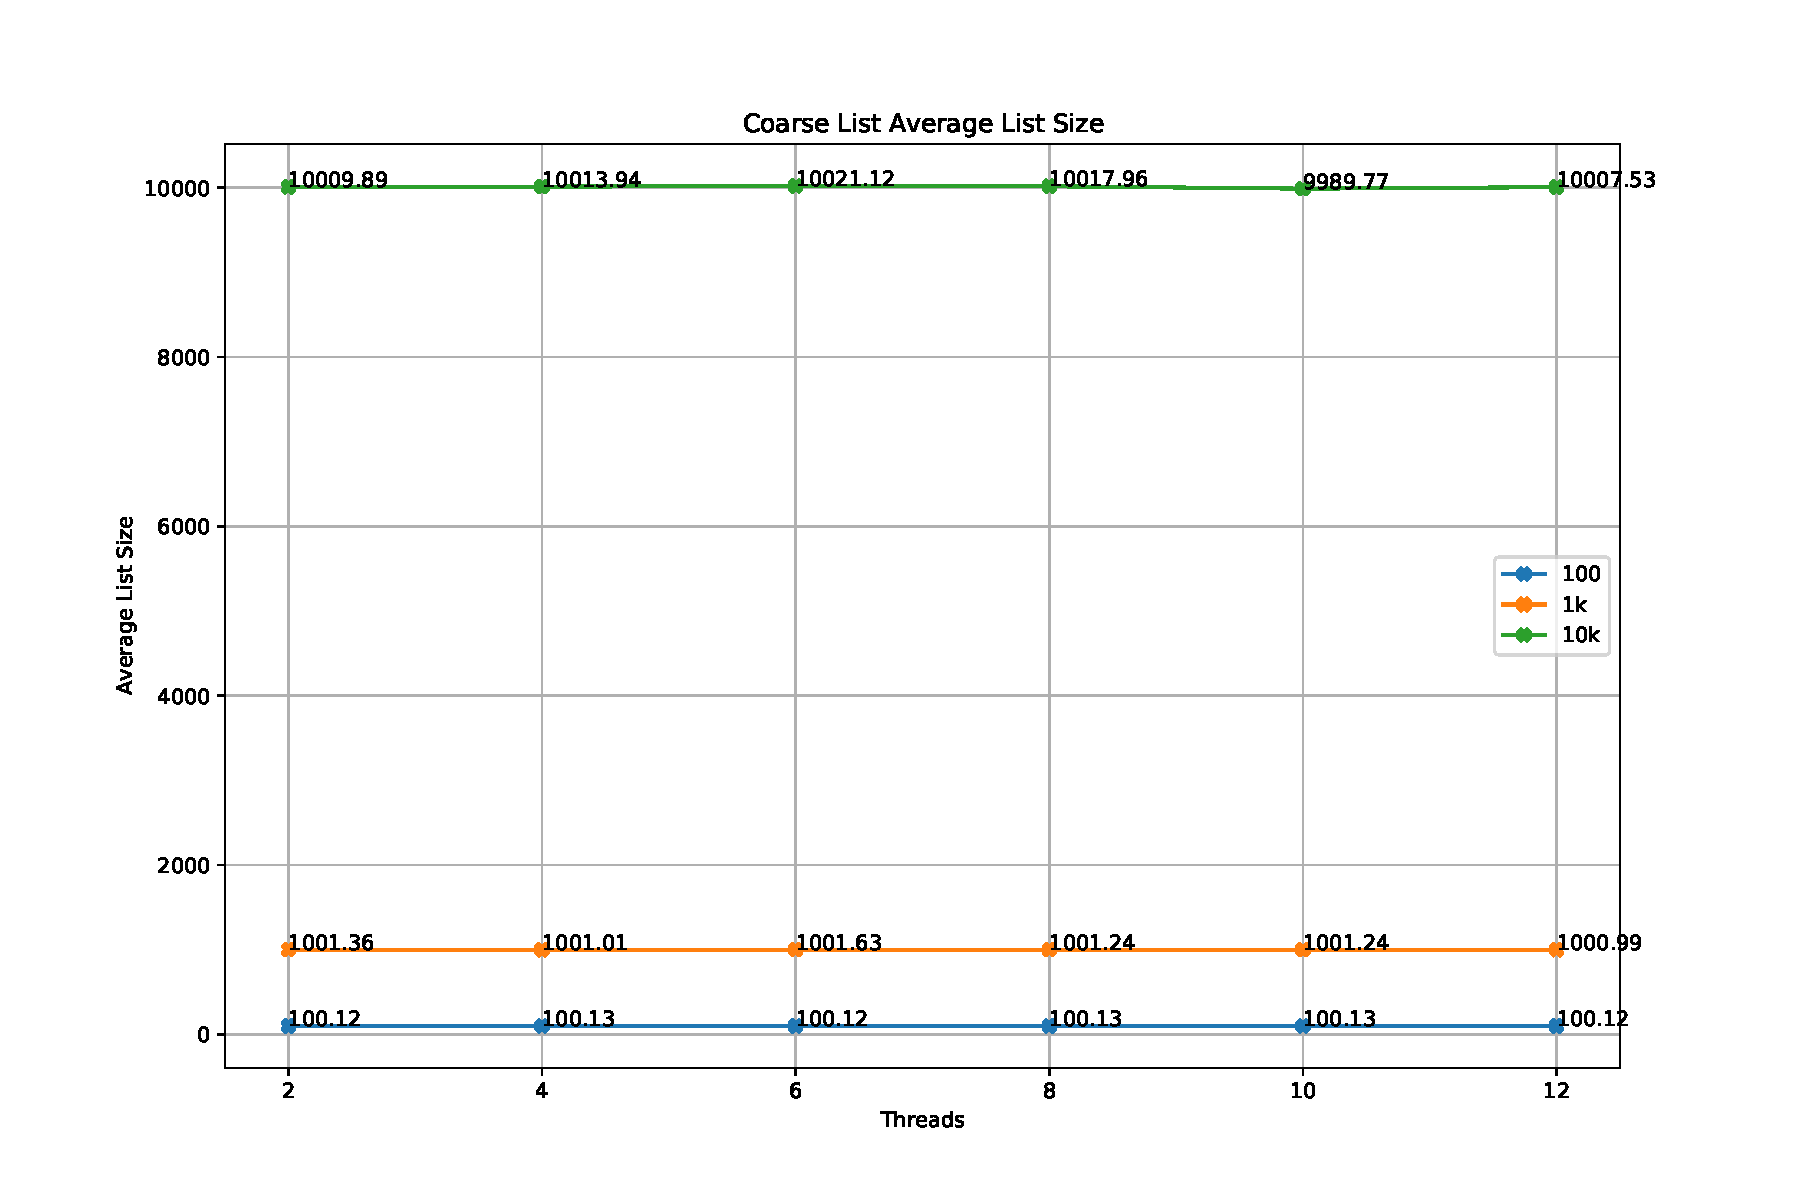
\includegraphics[scale=0.4]{../test/plots/CoarseListAverageListSize.pdf}
    \caption{Coarse List Average List Size}
    \label{fig:coarse-size}
\end{figure}

In general, what Figure~\ref{fig:coarse-throughput} shows is that increasing the number of threads does not increase the throughput. The list with 100 items had better performance with 4 threads and the worst performance with 12 threads. In a larger coarse list, the number of threads does not affect the throughput.

\begin{figure}[H]
    \centering
    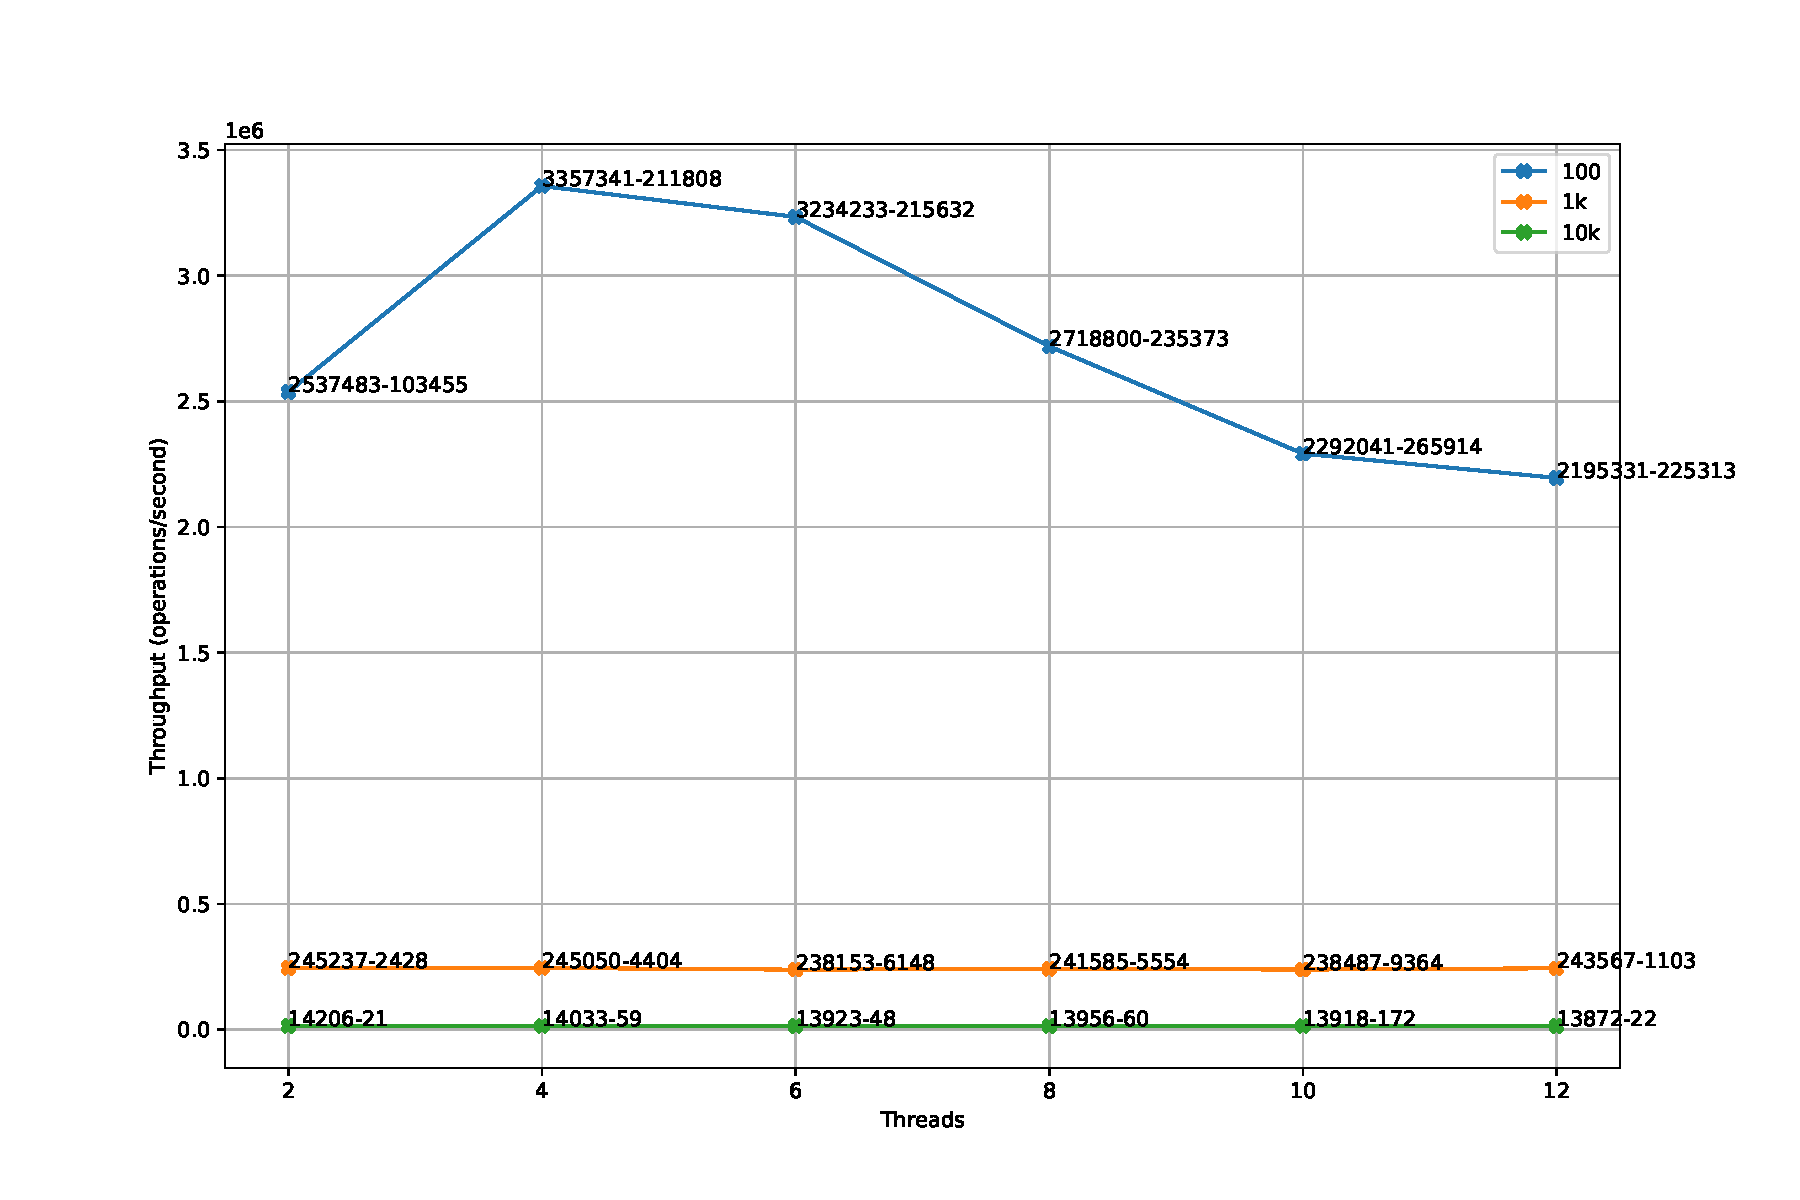
\includegraphics[width=\textwidth]{../test/plots/CoarseListThroughput.pdf}
    \caption{Coarse List Throughput}
    \label{fig:coarse-throughput}
\end{figure}

\subsection{Fine list}

Figure~\ref{fig:fine-size} shows the average size of the fine list.

\begin{figure}[H]
    \centering
    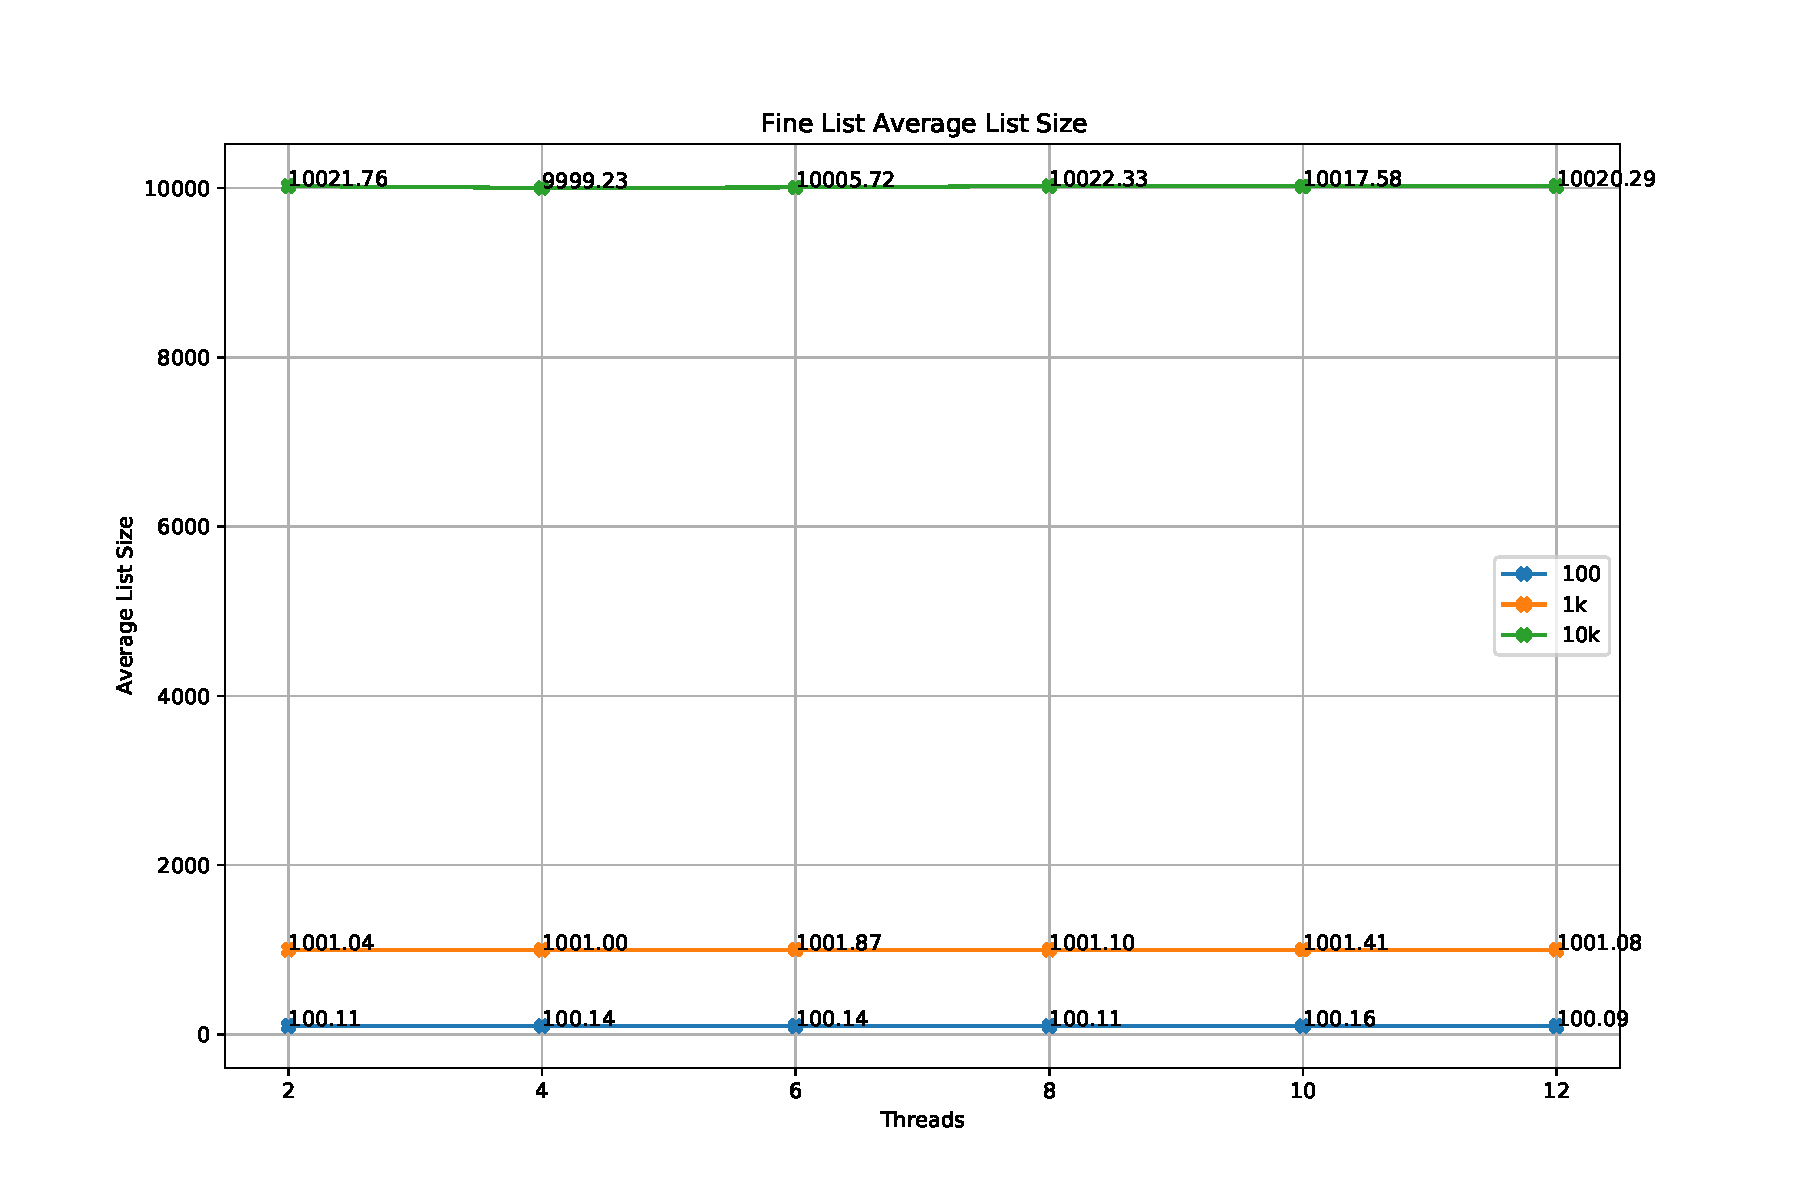
\includegraphics[scale=0.4]{../test/plots/FineListAverageListSize.pdf}
    \caption{Fine List Average List Size}
    \label{fig:fine-size}
\end{figure}

Similar to the coarse list, in general, increasing the number of threads does not increase throughput of the list. Only in the larger list, the throughput increased with the number of threads, as shown in Figure~\ref{fig:fine-throughput}.

A strange behavior happened in the list with 100 elements, using 2 threads. I do not know why, but the throughput was much higher than the same list size using 4 threads.

\begin{figure}[H]
    \centering
    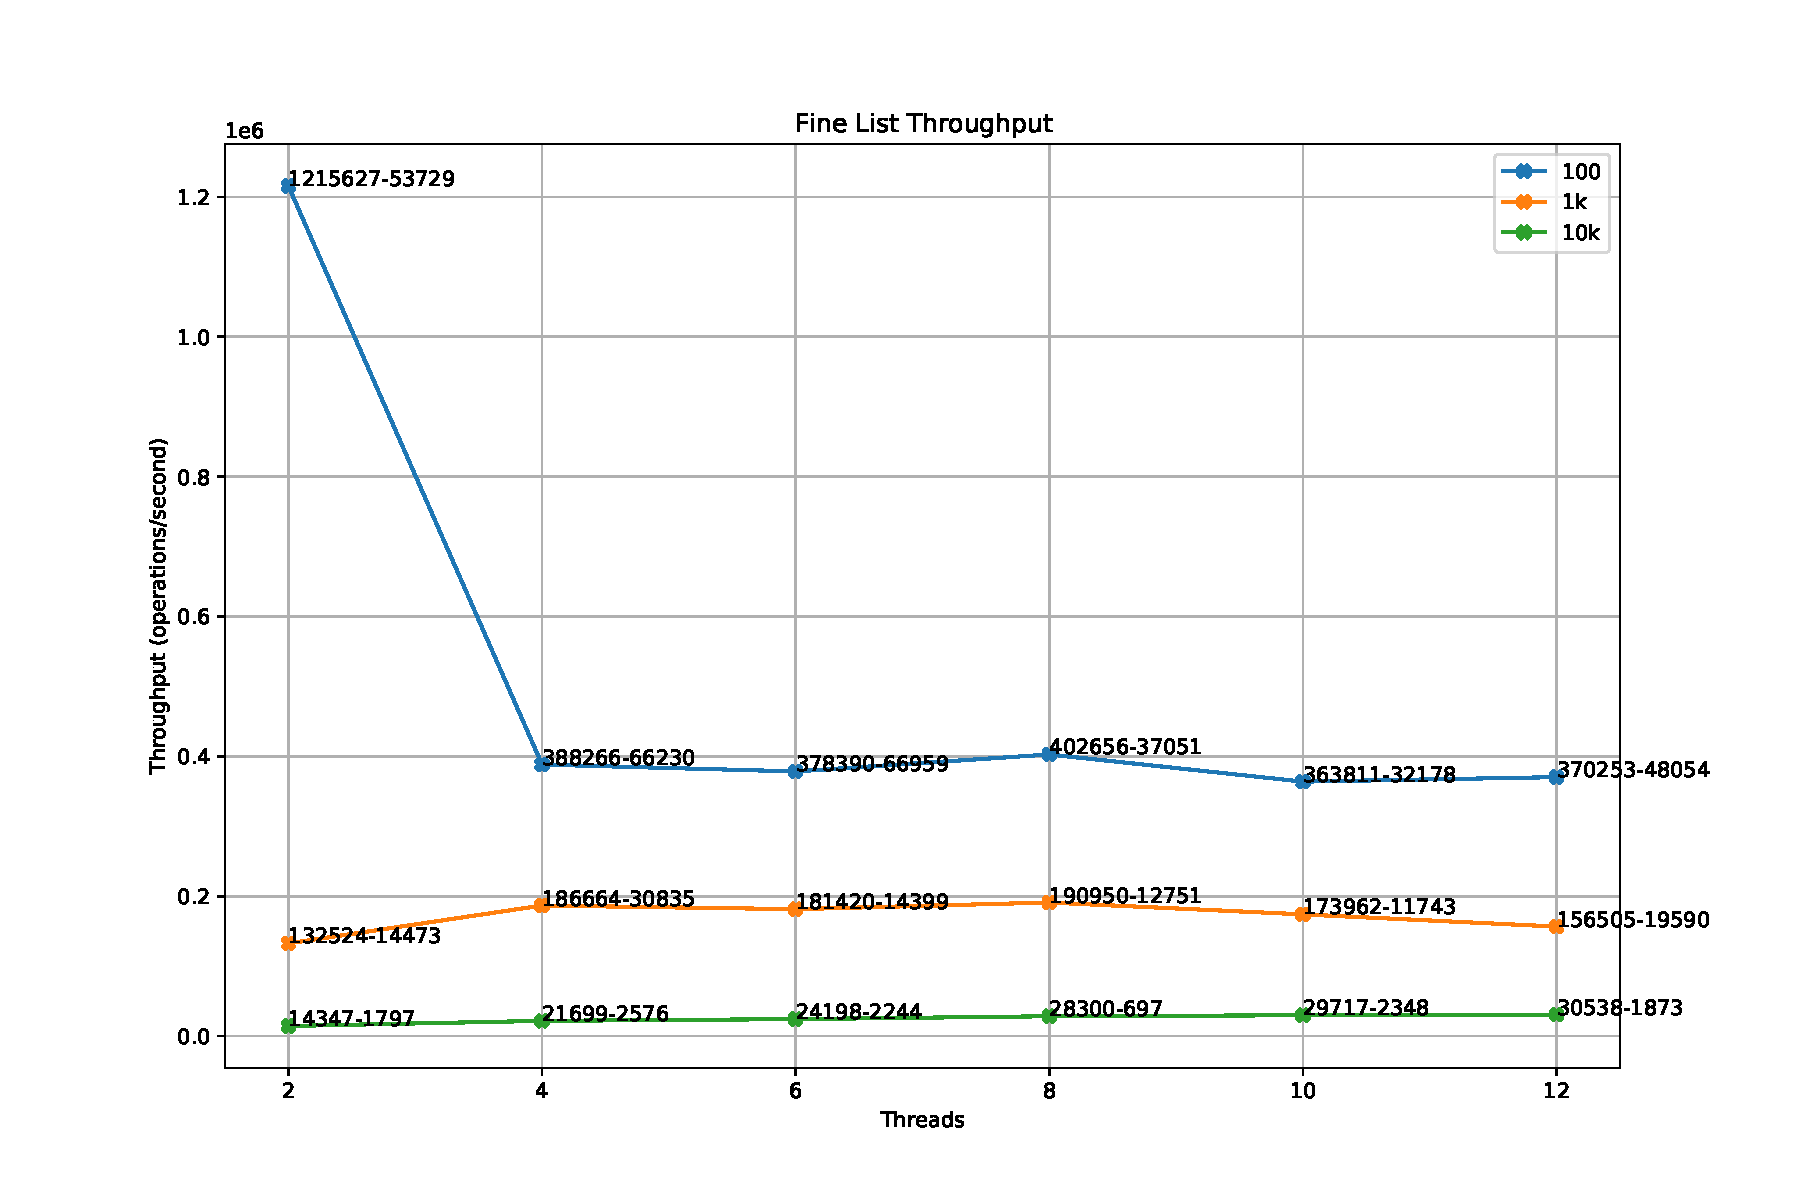
\includegraphics[width=\textwidth]{../test/plots/FineListThroughput.pdf}
    \caption{Fine List Throughput}
    \label{fig:fine-throughput}
\end{figure}

\subsection{Optimistic list}

Figure~\ref{fig:optimistic-size} shows the average size of the optimistic list.

\begin{figure}[H]
    \centering
    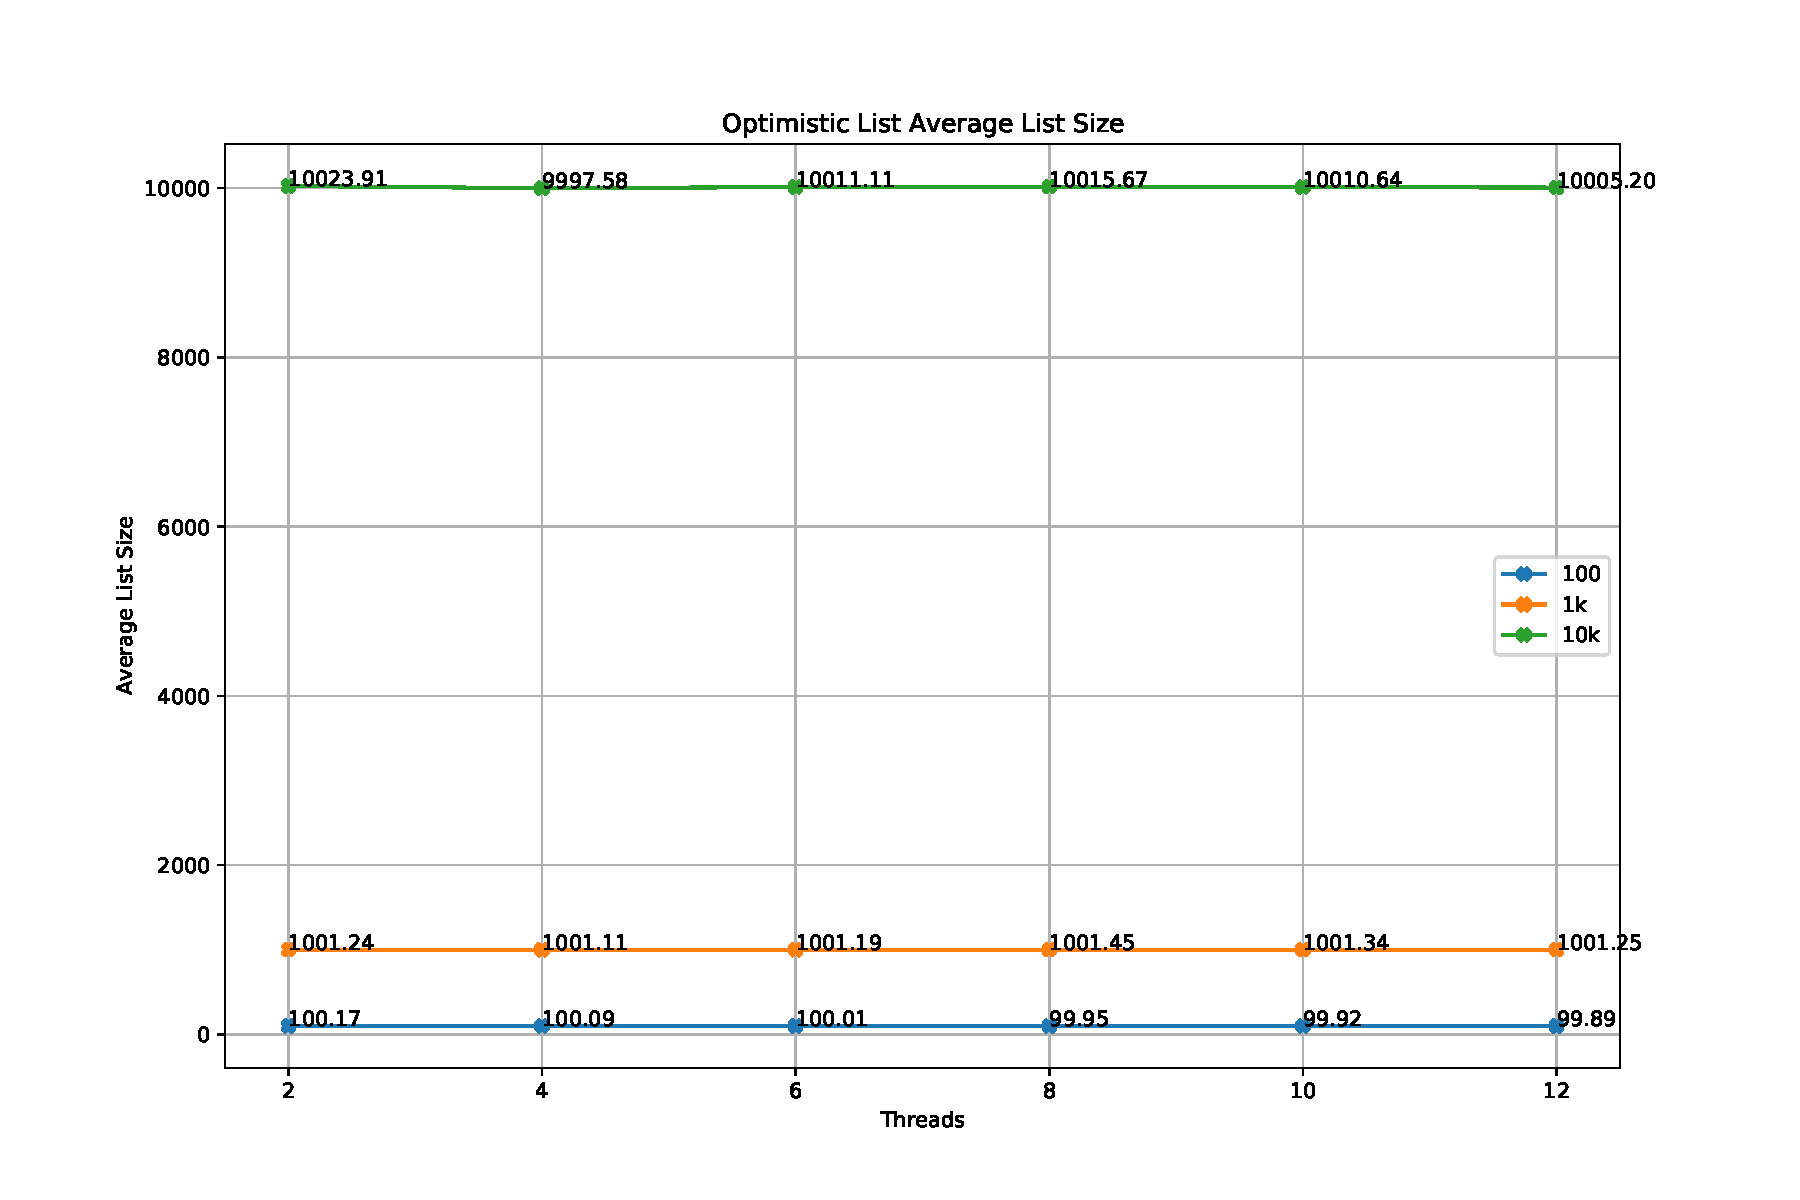
\includegraphics[scale=0.4]{../test/plots/OptimisticListAverageListSize.pdf}
    \caption{Optimistic List Average List Size}
    \label{fig:optimistic-size}
\end{figure}

The list with 100 items decreased the performance with more threads. In the other two lists, more threads resulted in more throughput, as shown in Figure~\ref{fig:optimistic-throughput}.

\begin{figure}[H]
    \centering
    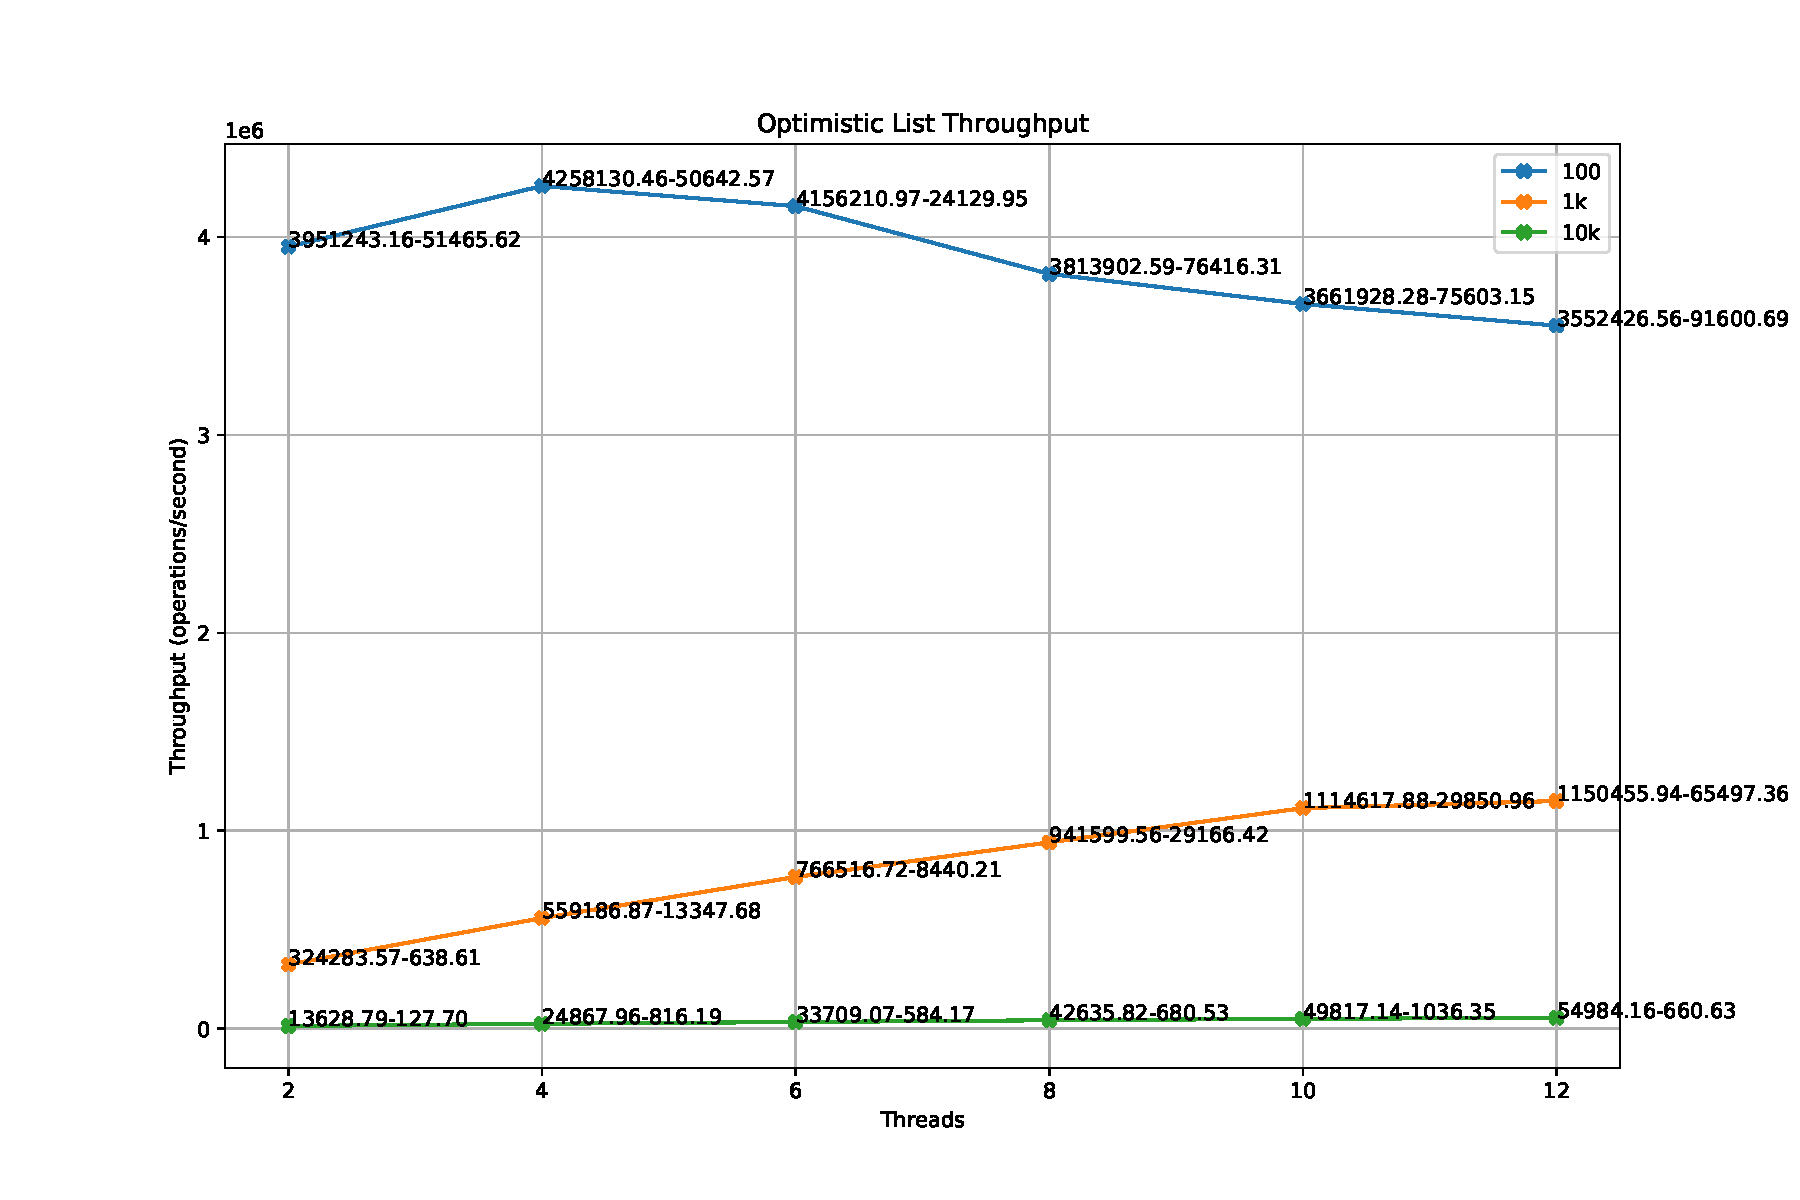
\includegraphics[width=\textwidth]{../test/plots/OptimisticListThroughput.pdf}
    \caption{Optimistic List Throughput}
    \label{fig:optimistic-throughput}
\end{figure}

\subsection{Lazy list}

Figure~\ref{fig:lazy-size} shows the average size of the lazy list.

\begin{figure}[H]
    \centering
    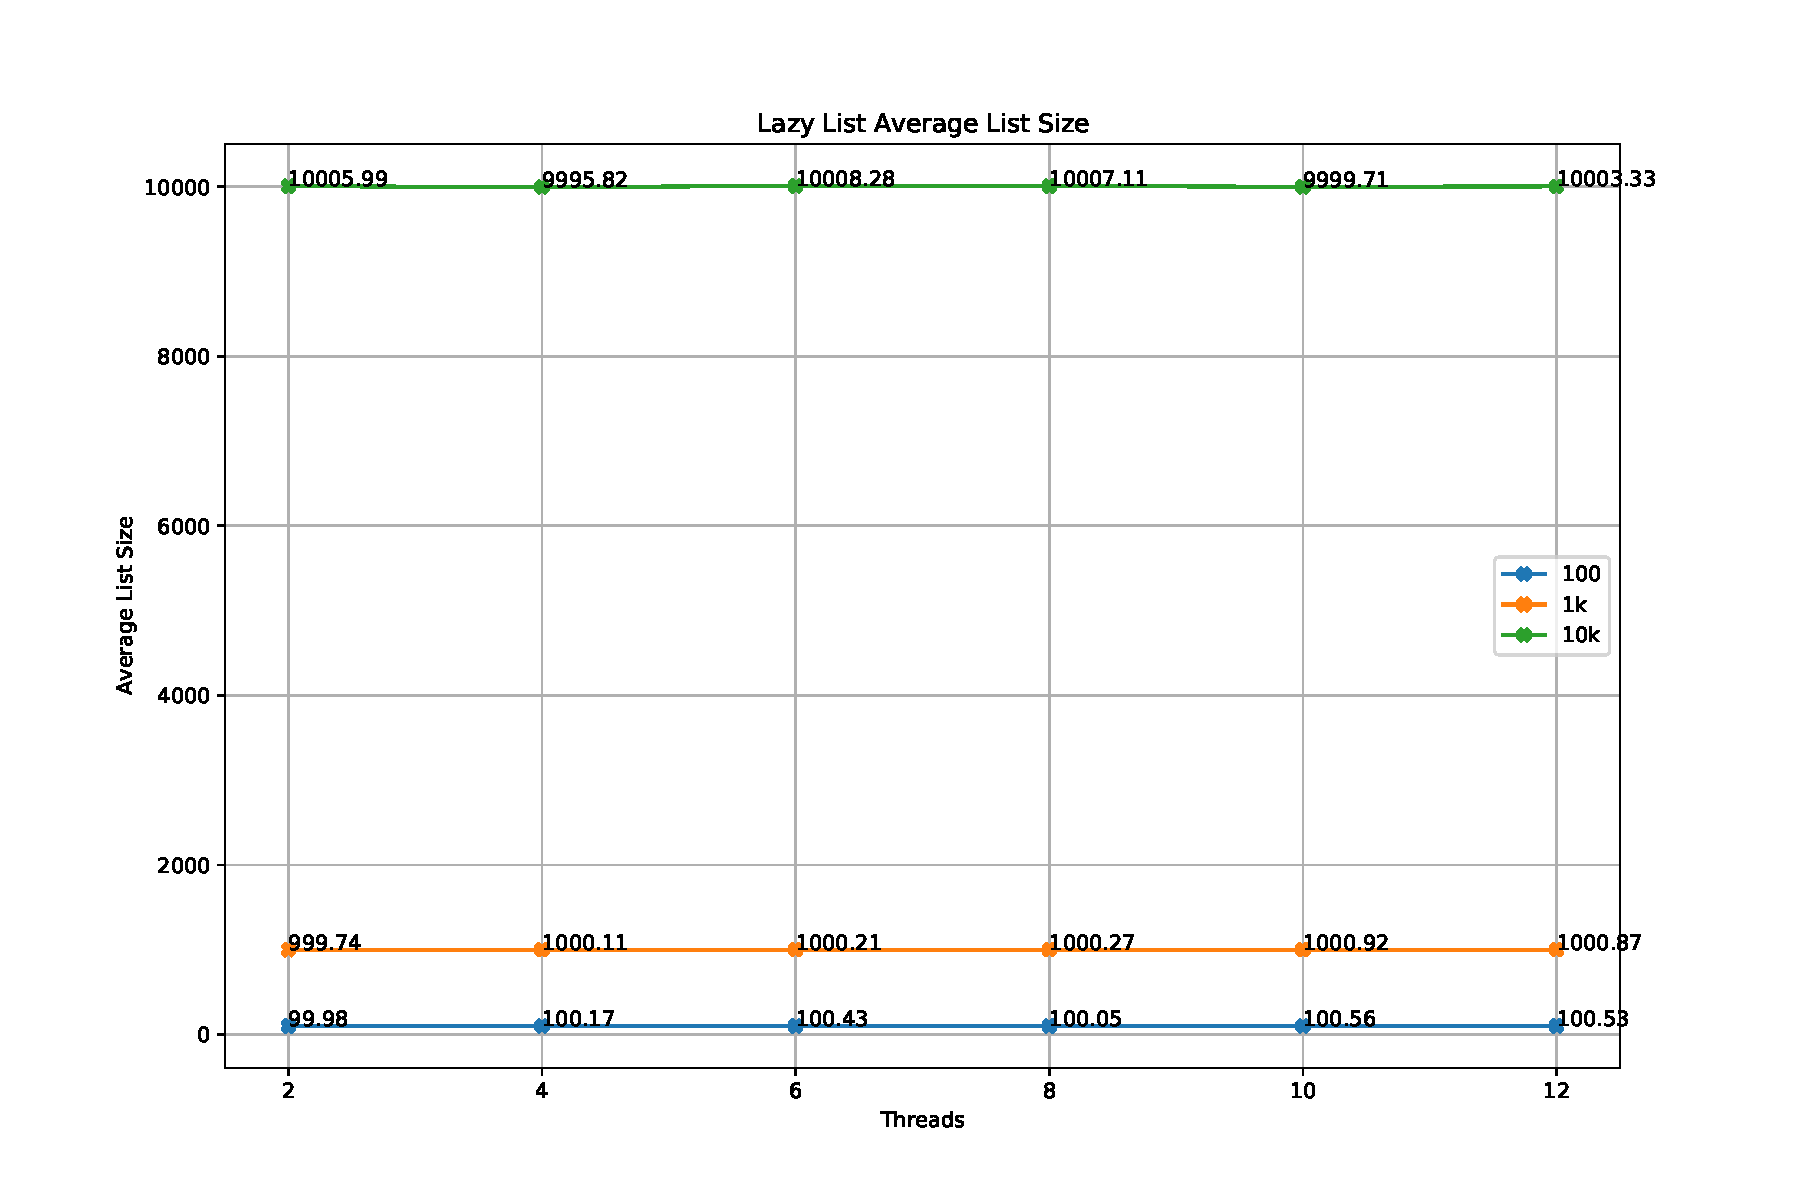
\includegraphics[scale=0.4]{../test/plots/LazyListAverageListSize.pdf}
    \caption{Lazy List Average List Size}
    \label{fig:lazy-size}
\end{figure}

Among the list that used a lock mechanism, the lazy list had the best performance. With the smaller list, the throughput increased up to 8 threads and, considering the standard deviation, the throughput was almost stable with 10 and 12 threads.

With the larger lists, the throughput increased with the number of threads, as shown in Figure~\ref{fig:lazy-throughput}. On a computer with more CPUs available, the throughput may increase even more.

\begin{figure}[H]
    \centering
    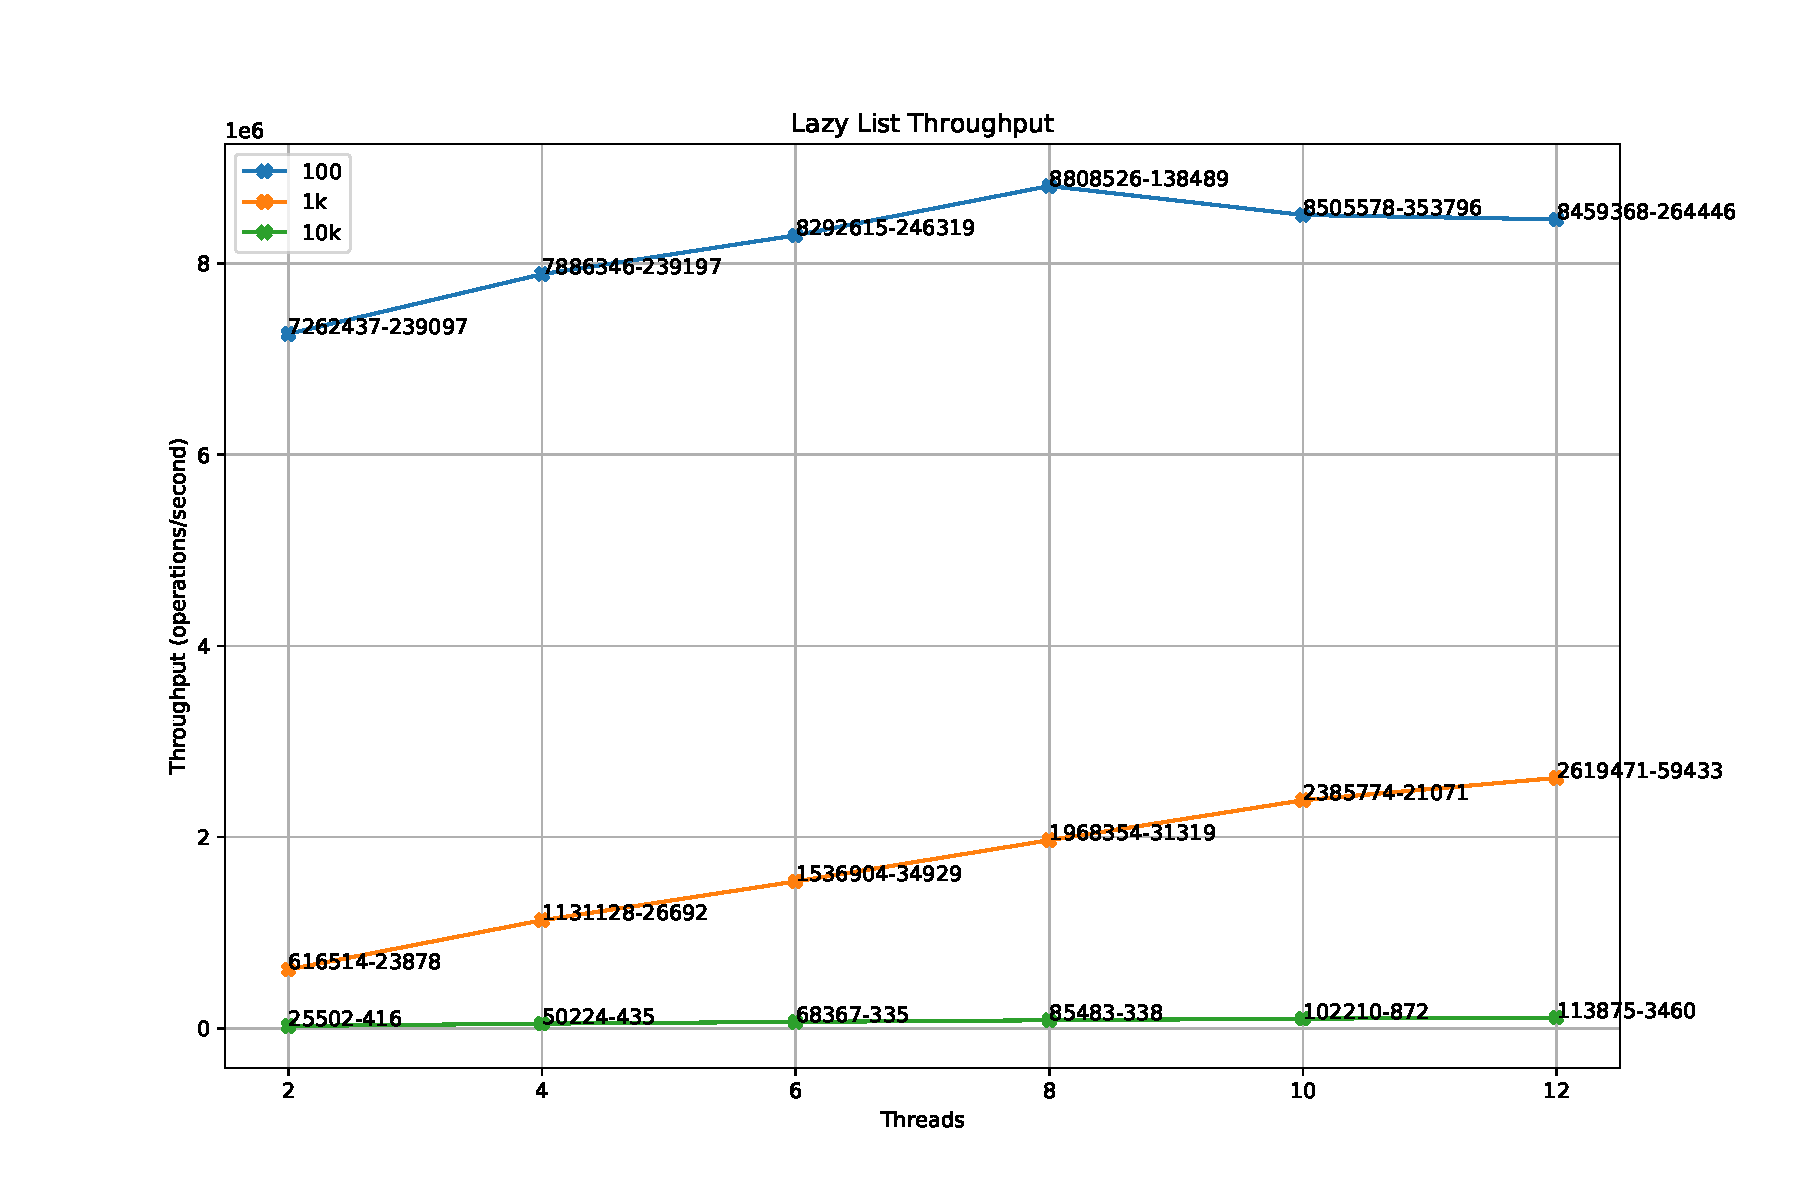
\includegraphics[width=\textwidth]{../test/plots/LazyListThroughput.pdf}
    \caption{Lazy List Throughput}
    \label{fig:lazy-throughput}
\end{figure}

\subsection{Lock free list}

Figure~\ref{fig:lock-free-size} shows the average size of the lock free list.

\begin{figure}[H]
    \centering
    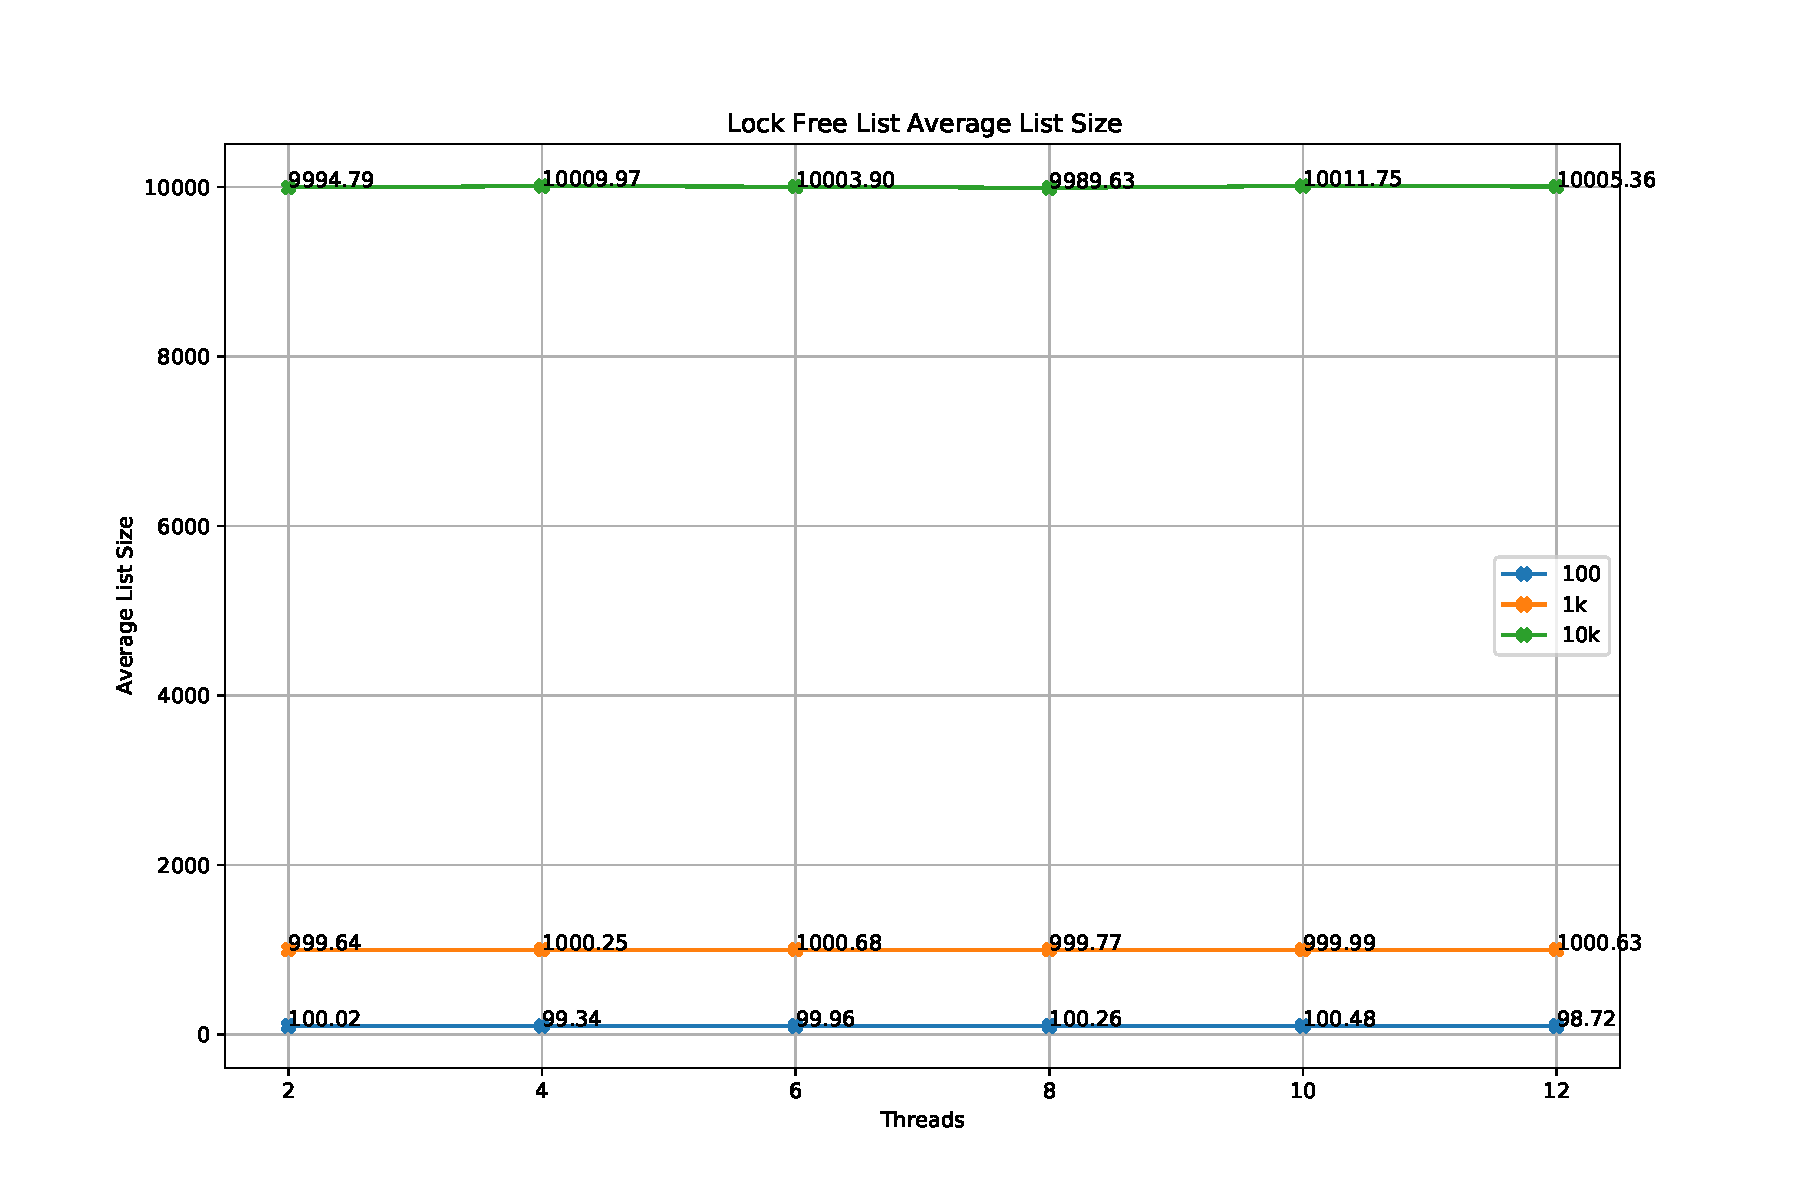
\includegraphics[scale=0.4]{../test/plots/LockFreeListAverageListSize.pdf}
    \caption{Lock Free List Average List Size}
    \label{fig:lock-free-size}
\end{figure}

The lock free list, as the name implies, does not use the lock mechanism. Therefore, intuitively, it is expected to have a higher throughput. However, as Figure~\ref{fig:lock-free-throughput} shows, the lock free list surpasses the lazy list only in smaller lists. As the number of items in the list increases, the throughput of tje optimistic list becomes worst than when using the lock mechanism.

Even so, it is important to note than the throughput increases significantly with the number of threads.

\begin{figure}[H]
    \centering
    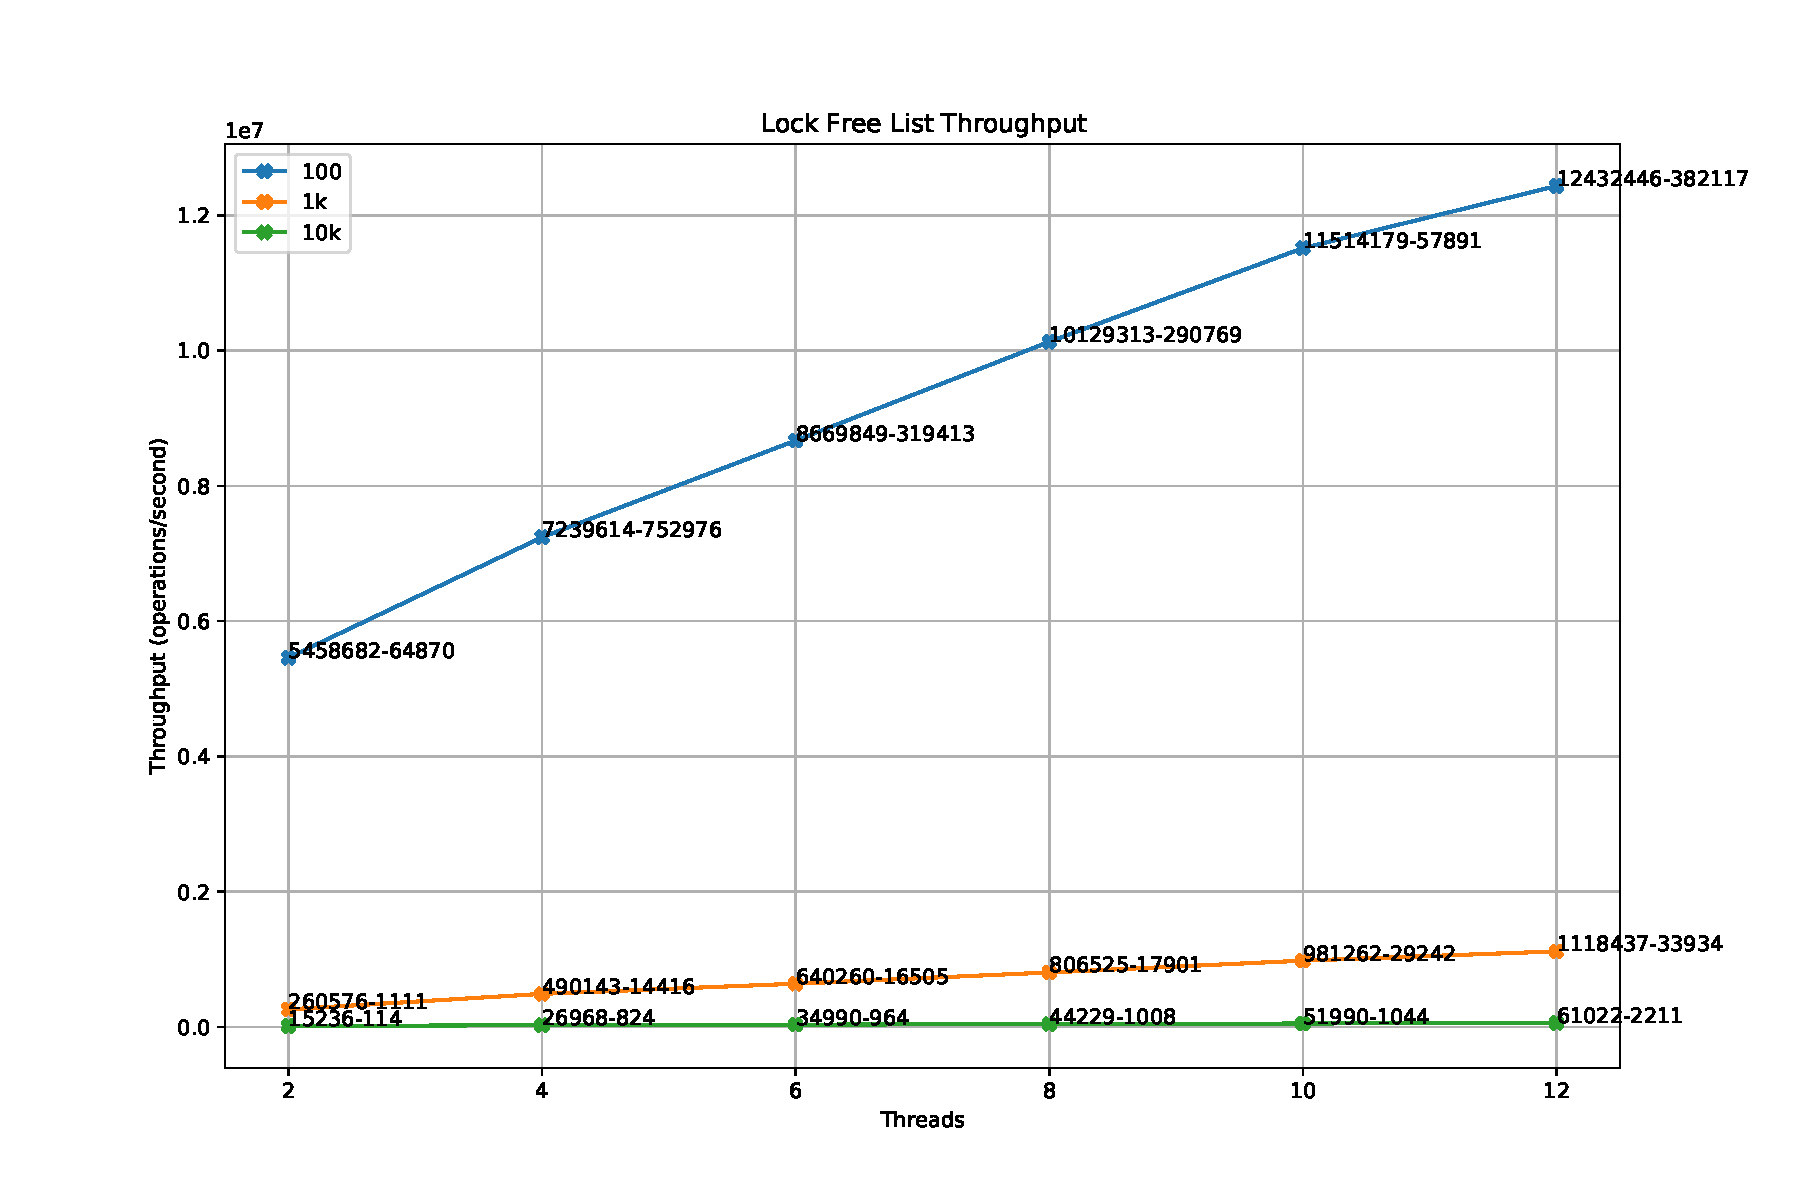
\includegraphics[width=\textwidth]{../test/plots/LockFreeListThroughput.pdf}
    \caption{Lock Free List Throughput}
    \label{fig:lock-free-throughput}
\end{figure}


\section{Conclusions}

The lock free list have a good performance on small lists. However, on a larger list, its performance can be poor when compared to the lazy list. One possible explanation for this is that the list needs many while loops to ensure that a node was not changed by another thread.

In general, as the number of threads increase, the throughput also increases. Another important thing to note is that, as the complexity of the list increases, the throughput also increases. This shows that there is space for new approaches that make a better use of the resources provided by the computer or even by the programming language.


\section{Source code} \label{sec:source-code}

All the souce code used in this work are available here: \url{https://github.com/claudioscheer/concurrent-producer-consumer}.


\bibliographystyle{unsrt}
\bibliography{references}

\end{document}